%%%%%%%%%%%%%%%%%%%%%%%%%%%%%%%%%%%%%%%%%%%%%%%%%%%%%%%%%%%%%%%%%%%%%%%%%%%%%%%%
\section{Interpretação corporal da música}
Seguindo a Definição \ref{def:MusicalidadeNaDanca},
para que um dançarino tenha musicalidade, este precisa primeiro,
incorporar em si mesmo a informação que traz a música, 
este processo é chamado de \hyperref[cap:percepcaomusical]{\textbf{percepção musical}}, 
e ja foi abordado no Capítulo \ref{cap:percepcaomusical}.
Com esta informação, o dançarino deve procesar e escolher uma forma de interpretar corporalmente,
esta informação, ver Figura \ref{fig:interpretacion-corporal}.
\begin{figure}[!h]
  \centering
    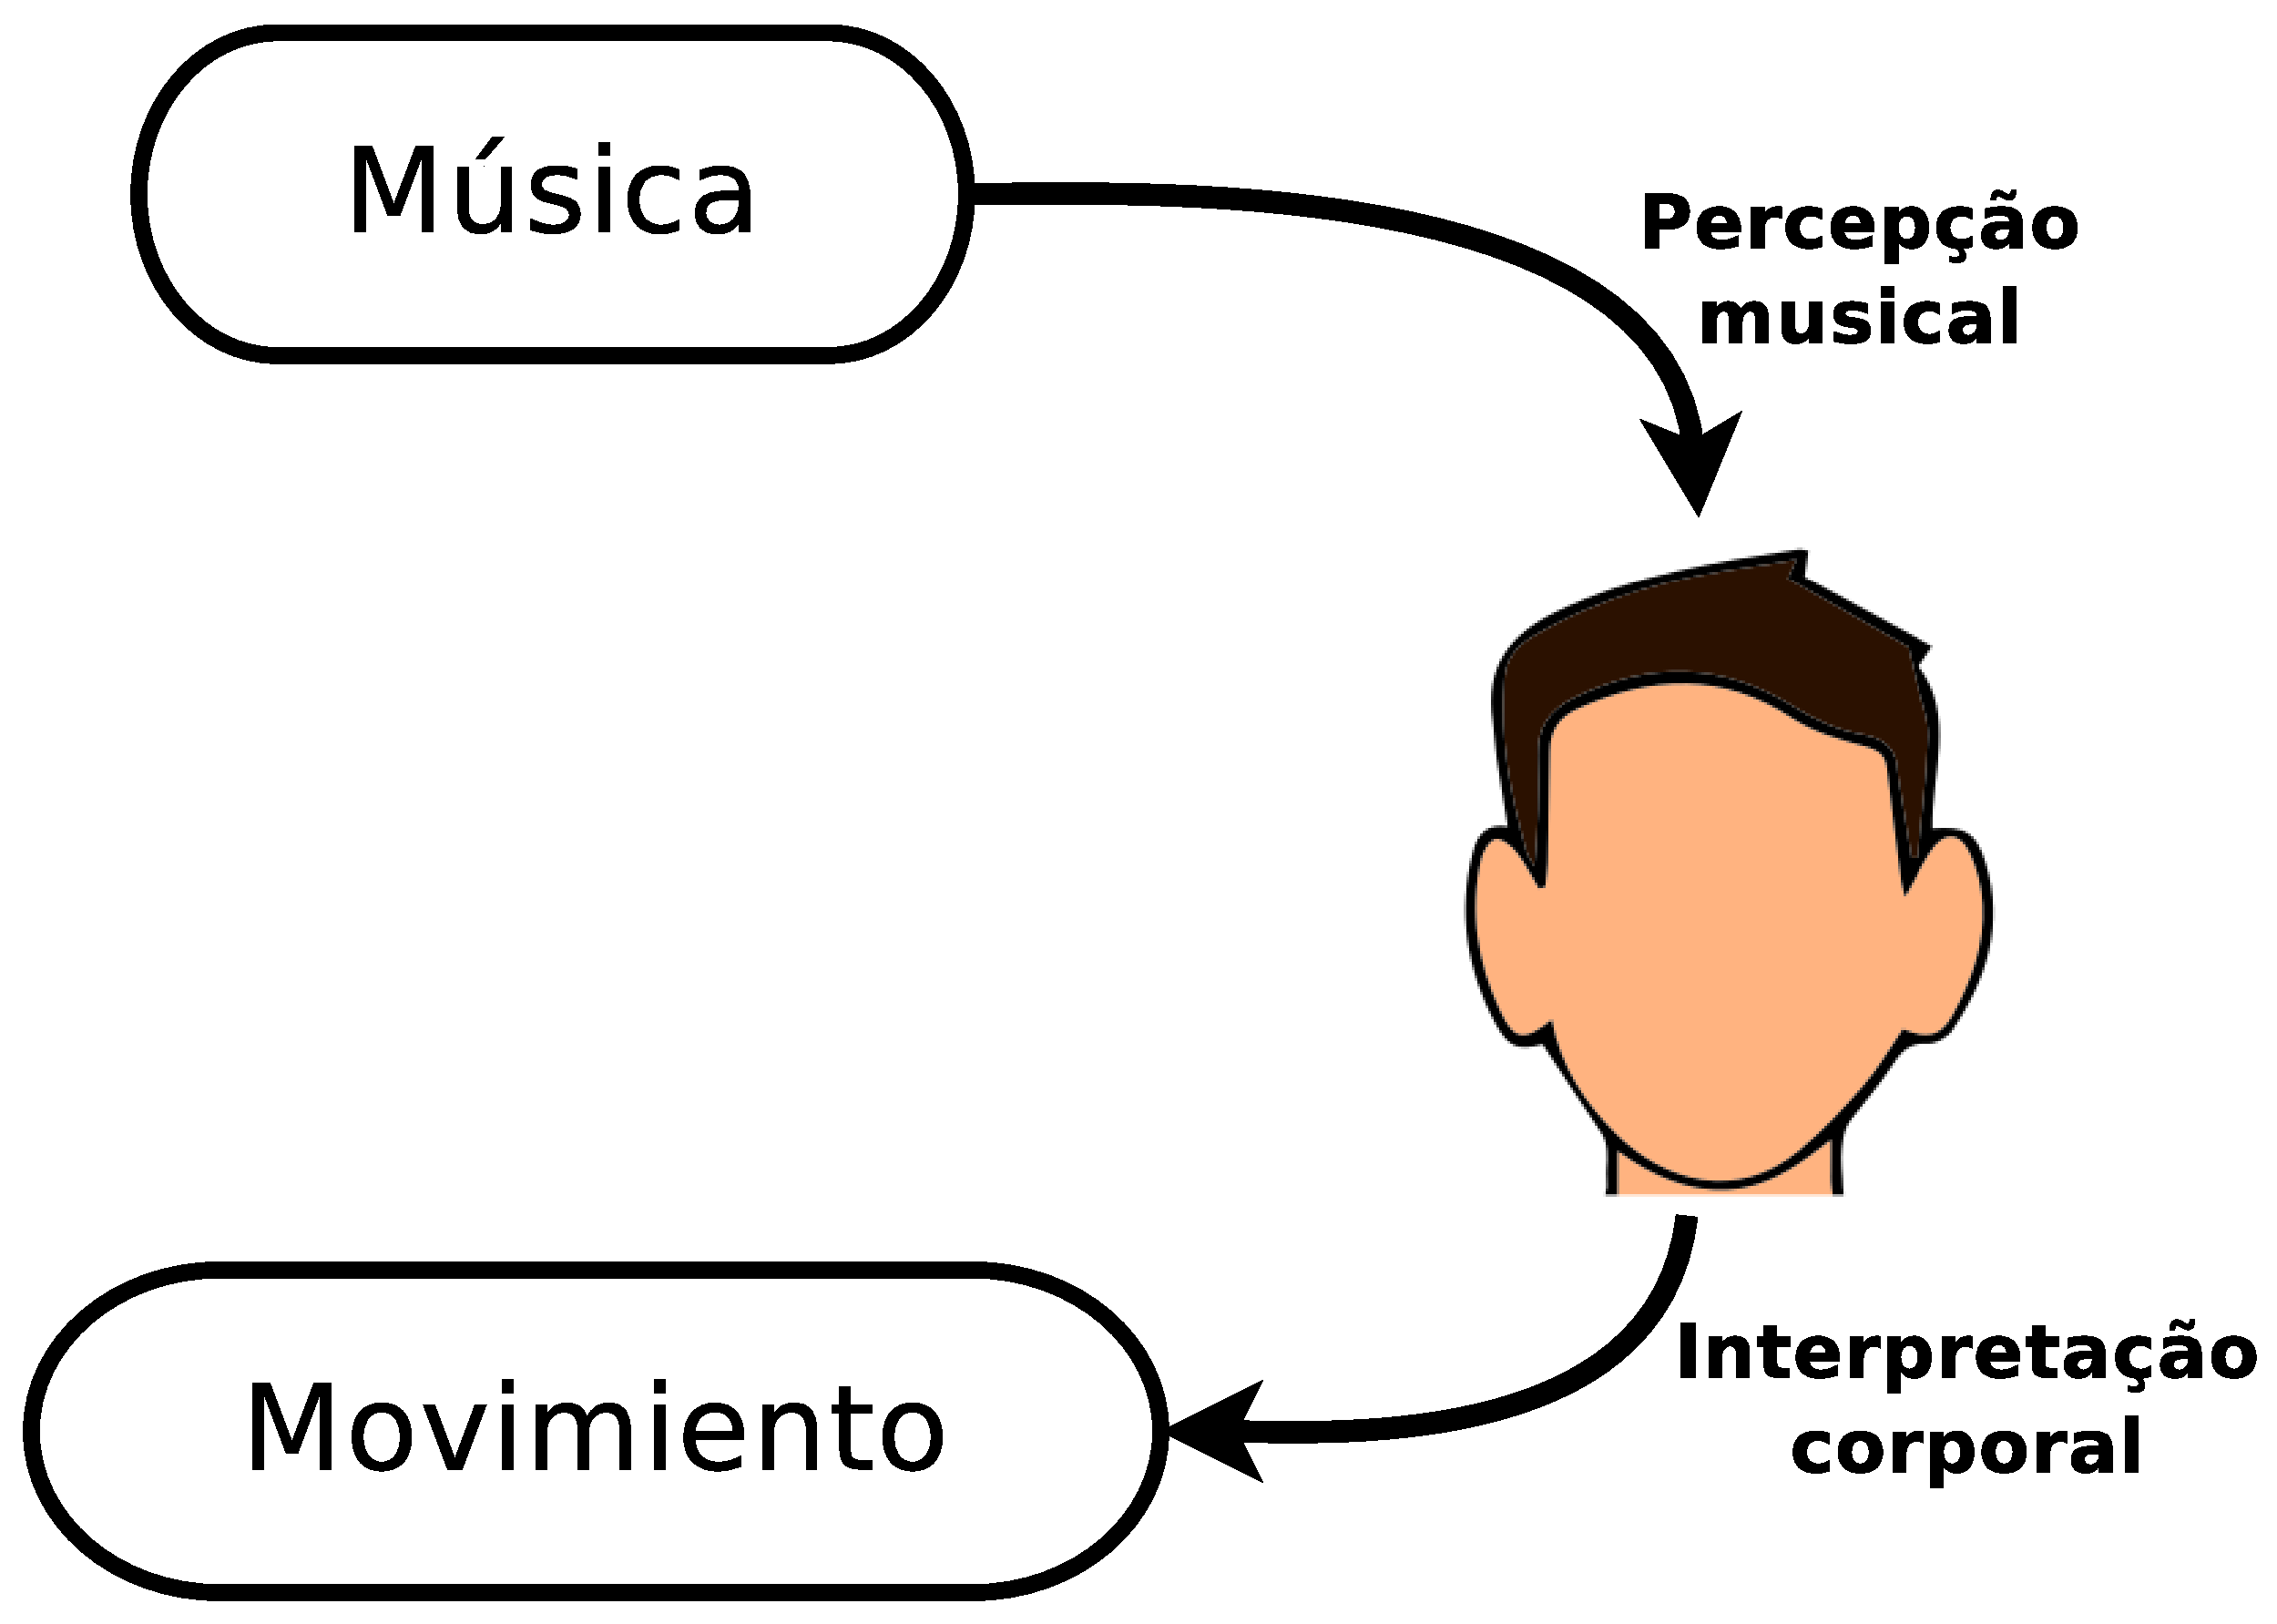
\includegraphics[width=1.00\textwidth]{chapters/cap-musicalidade/interpretacion-corporal.eps}
\caption{Interpretação corporal da música.}
\label{fig:interpretacion-corporal}
\end{figure}

As formas de como o dançarino interpreta esta informação estão amplamente estudadas,
não só no âmbito da dança, se não de forma geral no âmbito das artes cênicas;
entre os pontos de estudo, mais difundidos, 
para a interpretação de ideias  mediante o uso do corpo, podemos encontrar:
\begin{itemize}
\item A consciência corporal,
\item o controle corporal,
\item a dissociação corporal, e
\item a expressão corporal.
\end{itemize}
Para conhecer as definições e mais detalhes de como podemos aprimorar estes tópicos,
invito aos leitores a ir ao capítulo \ref{fig:bodyrelations}.

No caso da dança a dois, o dançarino usa todos estes elementos, 
para enviar ou projetar corporalmente uma informação, que tenha coerência com a música que percebe.
Os receptores ou destinatários destas informações, podem ser: o par de dança,
o público, ou o próprio dançarino; 
assim, dependendo do âmbito em que este se desenvolva,
podem incluso ser todos eles, ao mesmo tempo, os receptores da informação.

É neste ponto que o dançarino tem mais liberdade criativa, 
e onde podem ser introduzidas subjetividades; por exemplo,
se a ideia ou informação recopilada pelo dançarino está representada pela Figura \ref{fig:LaCopaDeRubin};
este interpretará um  movimento de bêbados ou de namorados?
\begin{figure}[!h]
  \centering
    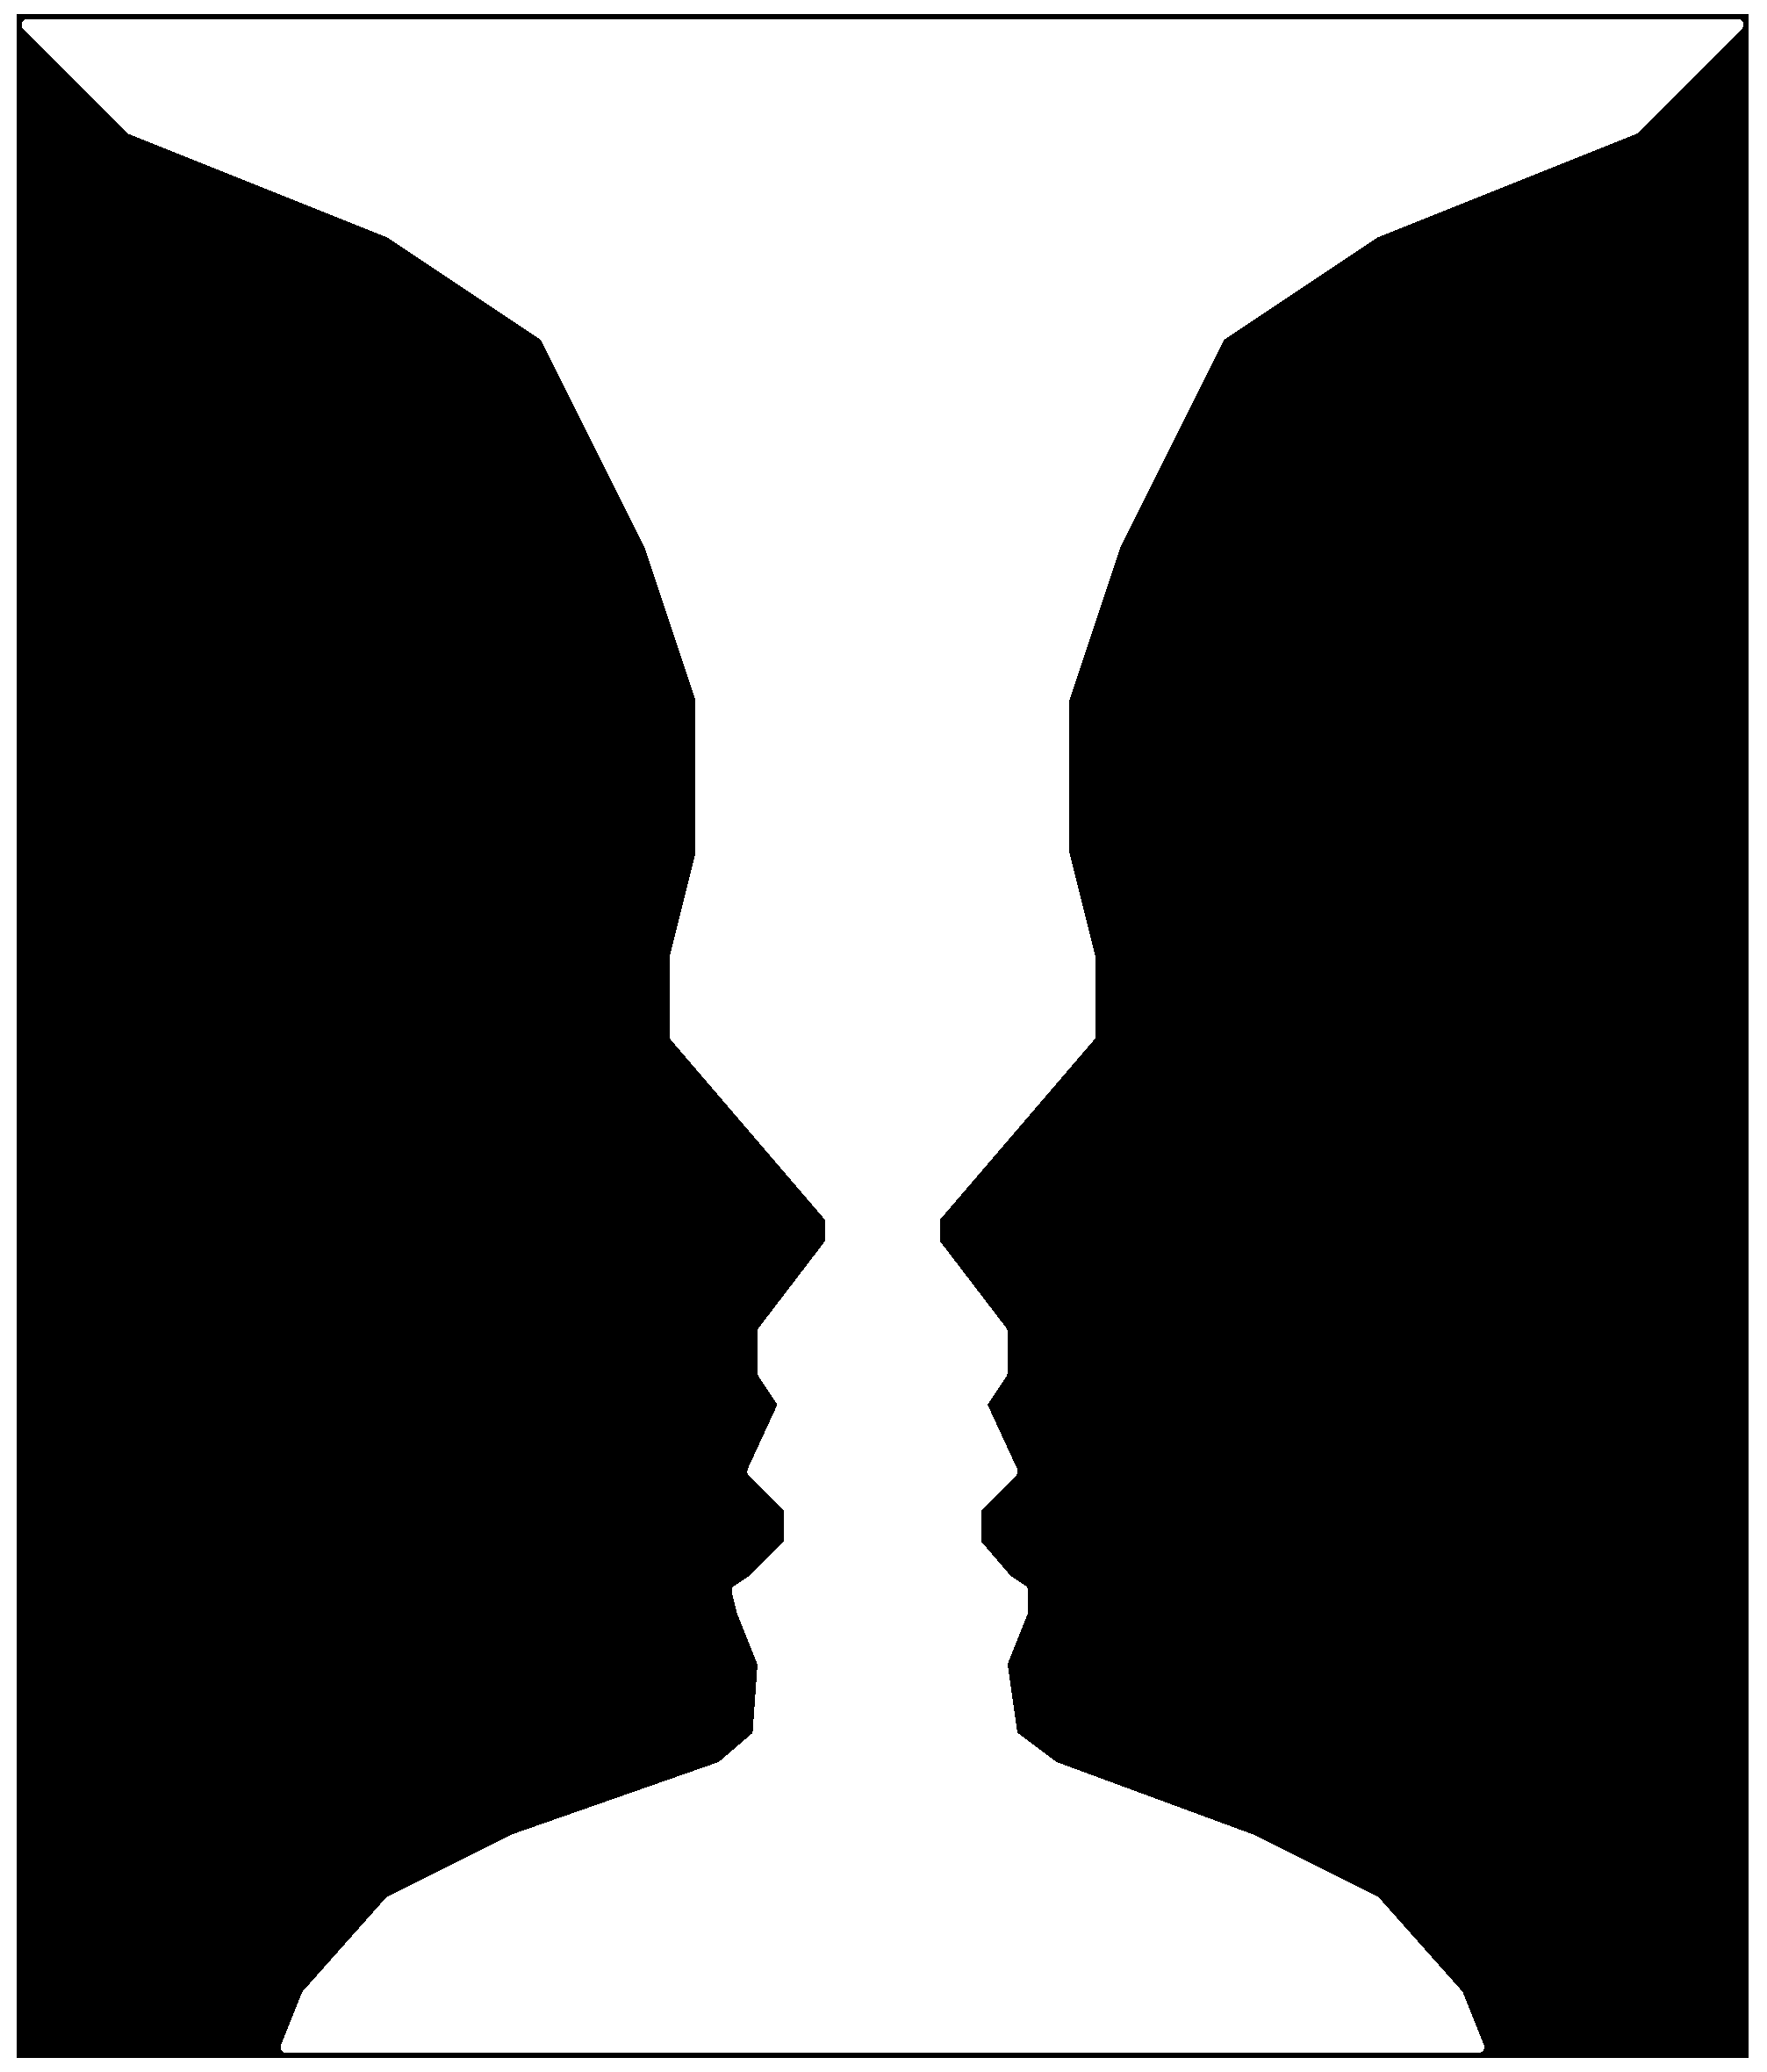
\includegraphics[width=0.5\textwidth]{chapters/cap-musicalidade/LaCopaDeRubin.eps}
\caption{Aperspetiva do interprete.}
\label{fig:LaCopaDeRubin}
\end{figure}

O objetivo deste capítulo e dos seguintes, não é indicar se na Figura \ref{fig:LaCopaDeRubin},
existe uma copa ou duas pessoas se olhando frente a frente; e sim desenvolver técnicas ou 
apresentar treinamentos para projetar qualquer destas duas perspetivas, seguindo a interpretação de cada dançarino.



